%%%%%%%%%%%%%%%%%%%%%%%%%%%%%%%%%%%%%%%
% Header                              %
%%%%%%%%%%%%%%%%%%%%%%%%%%%%%%%%%%%%%%%
% 
% Revisions: 2017-12-12 Martin Raedel <martin.raedel@dlr.de>
%                       Initial draft
%               
% Contact:   Martin Raedel,  martin.raedel@dlr.de
%            DLR Composite Structures and Adaptive Systems
%          
%                                 __/|__
%                                /_/_/_/  
%            www.dlr.de/fa/en      |/ DLR
% 
%%%%%%%%%%%%%%%%%%%%%%%%%%%%%%%%%%%%%%%
% Content                             %
%%%%%%%%%%%%%%%%%%%%%%%%%%%%%%%%%%%%%%%

%   \settoheight\figdim{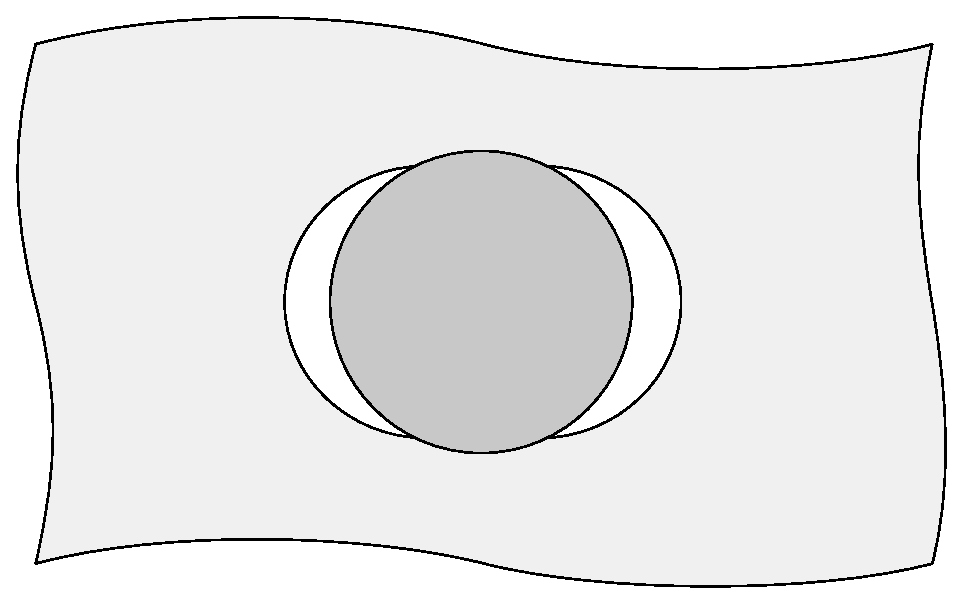
\includegraphics[width=\figwidth,height=\figheight,keepaspectratio]{Obs_Model_Single_Fiber}}
  \savebox{\largestimage}{%%%%%%%%%%%%%%%%%%%%%%%%%%%%%%%%%%%%%%%
% Header                              %
%%%%%%%%%%%%%%%%%%%%%%%%%%%%%%%%%%%%%%%
% 
% Revisions: 2017-12-12 Martin Raedel <martin.raedel@dlr.de>
%                       Initial draft
%               
% Contact:   Martin Raedel,  martin.raedel@dlr.de
%            DLR Composite Structures and Adaptive Systems
%          
%                                 __/|__
%                                /_/_/_/  
%            www.dlr.de/fa/en      |/ DLR
% 
%%%%%%%%%%%%%%%%%%%%%%%%%%%%%%%%%%%%%%%
% Content                             %
%%%%%%%%%%%%%%%%%%%%%%%%%%%%%%%%%%%%%%%

\def\numarrows{9} % one more arrow is created

% \def\failureangle{73.25}
% \def\fibreradius{0.248}
\def\failureangle{64}
% \def\fibreradius{1.12}
\def\fibreradius{0.95}

\begin{tikzpicture}[
  every node/.style={font=\figurefontsize}
]
  % External figure
  \node[anchor=south west,inner sep=0] (image) at (0,0) {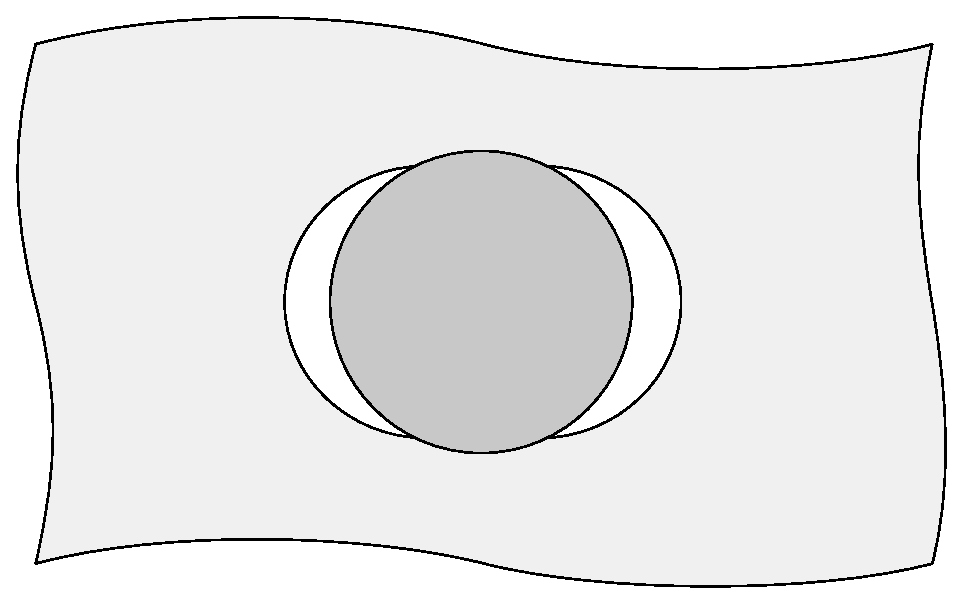
\includegraphics[width=\figwidth,height=\figheight,keepaspectratio]{Obs_Model_Single_Fiber}};
  % Relative node positioning to picture
  % \node[anchor=east] (impactorlabel) at ($(image.west)       + (-0.5cm, 0.5)$) {Impactor};
  % \node[anchor=west] (disklabel)     at ($(image.south east) + ( 0.5cm,0.5)$) {Disk};
  % Figure scope
  \begin{scope}[
    x={(image.south east)},
    y={(image.north west)},
  ]
    
    % Load arrows
    \foreach \y in {0,1,...,\numarrows} {\draw[-latex] (-0.025,\y/\numarrows) -- (-0.1,\y/\numarrows) coordinate (loadarrowleft\y);}
    \foreach \y in {0,1,...,\numarrows} {\draw[-latex] ( 1.025,\y/\numarrows) -- ( 1.1,\y/\numarrows) coordinate (loadarrowright\y);}
    
    % Load label
    \node[anchor=east] (loadlabelleft)  at (loadarrowleft0  |- 0,0.5) {$\glssymbol{symb:scalar:mech:stress:normal:engineering}_x$};
    \node[anchor=west] (loadlabelright) at (loadarrowright0 |- 0,0.5) {$\glssymbol{symb:scalar:mech:stress:normal:engineering}_x$};
    
    % Fibre-Matrix Label
    \node[anchor=south west,inner sep=1pt] (matrixlabel) at (0.05,0.1) {Matrix};
    \node[anchor=north west,inner sep=1pt] (fibrelabel)  at (0.51,0.9) {Fibre};
    \draw[thin] (fibrelabel) -- (0.525,0.725);
    
    % Crack opening
    \draw[thin,latex-latex] (0.66,0.5) -- (0.715,0.5) node[midway,below]{$\glssymbol{symb:scalar:geo:separation}$};
    
    % Fibre diameters
    \draw[dashed] (0.34,0.3) -- (0.34,0.15) coordinate[pos=0.8] (fibrediameterleft);
    \draw[dashed] (0.66,0.3) -- (0.66,0.15) coordinate[pos=0.8] (fibrediameterright);
    \draw[thin,latex-latex] (fibrediameterleft) -- (fibrediameterright) node[midway,below]{$\glssymbol{symb:scalar:geo:diameter}$};
    
    % Help grid and labels
    %\pic{myimagegrid};
  \end{scope}
    
  % Things that are influenced by the aspect ratio
  %\coordinate (fibreorigin) at (0.5,0.5);
  \coordinate (fibreorigin) at ($(image.south east)!0.5!(image.north west)$);
  \draw[thin,dashed] (fibreorigin) -- ++( \failureangle:\fibreradius) coordinate[pos=0.75] (failrt);
  \draw[thin,dashed] (fibreorigin) -- ++(-\failureangle:\fibreradius) coordinate[pos=0.75] (failrb);
  \draw[thin, latex-latex] (fibreorigin) ++(-\failureangle:0.8*\fibreradius) arc (-\failureangle:\failureangle:0.8*\fibreradius) node[midway,left]{$2\glssymbol{symb:scalar:geo:angle:debonding}$};

\end{tikzpicture}}
  %\settoheight\figdim{%%%%%%%%%%%%%%%%%%%%%%%%%%%%%%%%%%%%%%%
% Header                              %
%%%%%%%%%%%%%%%%%%%%%%%%%%%%%%%%%%%%%%%
% 
% Revisions: 2017-12-12 Martin Raedel <martin.raedel@dlr.de>
%                       Initial draft
%               
% Contact:   Martin Raedel,  martin.raedel@dlr.de
%            DLR Composite Structures and Adaptive Systems
%          
%                                 __/|__
%                                /_/_/_/  
%            www.dlr.de/fa/en      |/ DLR
% 
%%%%%%%%%%%%%%%%%%%%%%%%%%%%%%%%%%%%%%%
% Content                             %
%%%%%%%%%%%%%%%%%%%%%%%%%%%%%%%%%%%%%%%

\def\numarrows{9} % one more arrow is created

% \def\failureangle{73.25}
% \def\fibreradius{0.248}
\def\failureangle{64}
% \def\fibreradius{1.12}
\def\fibreradius{0.95}

\begin{tikzpicture}[
  every node/.style={font=\figurefontsize}
]
  % External figure
  \node[anchor=south west,inner sep=0] (image) at (0,0) {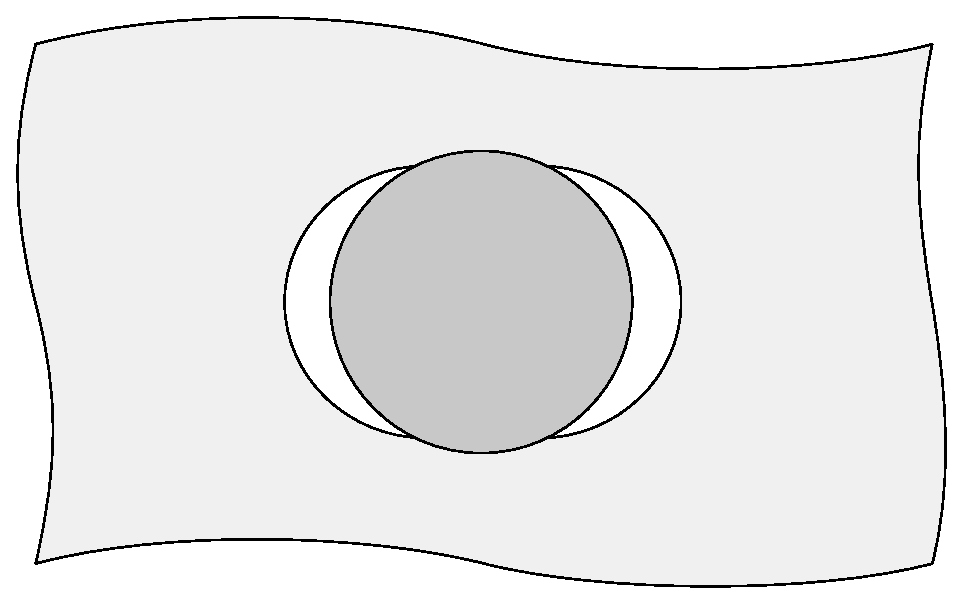
\includegraphics[width=\figwidth,height=\figheight,keepaspectratio]{Obs_Model_Single_Fiber}};
  % Relative node positioning to picture
  % \node[anchor=east] (impactorlabel) at ($(image.west)       + (-0.5cm, 0.5)$) {Impactor};
  % \node[anchor=west] (disklabel)     at ($(image.south east) + ( 0.5cm,0.5)$) {Disk};
  % Figure scope
  \begin{scope}[
    x={(image.south east)},
    y={(image.north west)},
  ]
    
    % Load arrows
    \foreach \y in {0,1,...,\numarrows} {\draw[-latex] (-0.025,\y/\numarrows) -- (-0.1,\y/\numarrows) coordinate (loadarrowleft\y);}
    \foreach \y in {0,1,...,\numarrows} {\draw[-latex] ( 1.025,\y/\numarrows) -- ( 1.1,\y/\numarrows) coordinate (loadarrowright\y);}
    
    % Load label
    \node[anchor=east] (loadlabelleft)  at (loadarrowleft0  |- 0,0.5) {$\glssymbol{symb:scalar:mech:stress:normal:engineering}_x$};
    \node[anchor=west] (loadlabelright) at (loadarrowright0 |- 0,0.5) {$\glssymbol{symb:scalar:mech:stress:normal:engineering}_x$};
    
    % Fibre-Matrix Label
    \node[anchor=south west,inner sep=1pt] (matrixlabel) at (0.05,0.1) {Matrix};
    \node[anchor=north west,inner sep=1pt] (fibrelabel)  at (0.51,0.9) {Fibre};
    \draw[thin] (fibrelabel) -- (0.525,0.725);
    
    % Crack opening
    \draw[thin,latex-latex] (0.66,0.5) -- (0.715,0.5) node[midway,below]{$\glssymbol{symb:scalar:geo:separation}$};
    
    % Fibre diameters
    \draw[dashed] (0.34,0.3) -- (0.34,0.15) coordinate[pos=0.8] (fibrediameterleft);
    \draw[dashed] (0.66,0.3) -- (0.66,0.15) coordinate[pos=0.8] (fibrediameterright);
    \draw[thin,latex-latex] (fibrediameterleft) -- (fibrediameterright) node[midway,below]{$\glssymbol{symb:scalar:geo:diameter}$};
    
    % Help grid and labels
    %\pic{myimagegrid};
  \end{scope}
    
  % Things that are influenced by the aspect ratio
  %\coordinate (fibreorigin) at (0.5,0.5);
  \coordinate (fibreorigin) at ($(image.south east)!0.5!(image.north west)$);
  \draw[thin,dashed] (fibreorigin) -- ++( \failureangle:\fibreradius) coordinate[pos=0.75] (failrt);
  \draw[thin,dashed] (fibreorigin) -- ++(-\failureangle:\fibreradius) coordinate[pos=0.75] (failrb);
  \draw[thin, latex-latex] (fibreorigin) ++(-\failureangle:0.8*\fibreradius) arc (-\failureangle:\failureangle:0.8*\fibreradius) node[midway,left]{$2\glssymbol{symb:scalar:geo:angle:debonding}$};

\end{tikzpicture}}
  \settoheight\figdim{\usebox{\largestimage}}
  \setlength{\figwidth}{\figwidth}
  \setlength{\figheight}{\figdim}
  %\global\setlength{\figwidth}{\figwidth}
  %\global\setlength{\figheight}{\figdim}
  % Figs
  \begin{subfigure}{0.59\linewidth}
    % Figure
    \centering
    \tikzexternalenable
    \tikzsetnextfilename{Obs_Model_Single_Fiber}
    %%%%%%%%%%%%%%%%%%%%%%%%%%%%%%%%%%%%%%%
% Header                              %
%%%%%%%%%%%%%%%%%%%%%%%%%%%%%%%%%%%%%%%
% 
% Revisions: 2017-12-12 Martin Raedel <martin.raedel@dlr.de>
%                       Initial draft
%               
% Contact:   Martin Raedel,  martin.raedel@dlr.de
%            DLR Composite Structures and Adaptive Systems
%          
%                                 __/|__
%                                /_/_/_/  
%            www.dlr.de/fa/en      |/ DLR
% 
%%%%%%%%%%%%%%%%%%%%%%%%%%%%%%%%%%%%%%%
% Content                             %
%%%%%%%%%%%%%%%%%%%%%%%%%%%%%%%%%%%%%%%

\def\numarrows{9} % one more arrow is created

% \def\failureangle{73.25}
% \def\fibreradius{0.248}
\def\failureangle{64}
% \def\fibreradius{1.12}
\def\fibreradius{0.95}

\begin{tikzpicture}[
  every node/.style={font=\figurefontsize}
]
  % External figure
  \node[anchor=south west,inner sep=0] (image) at (0,0) {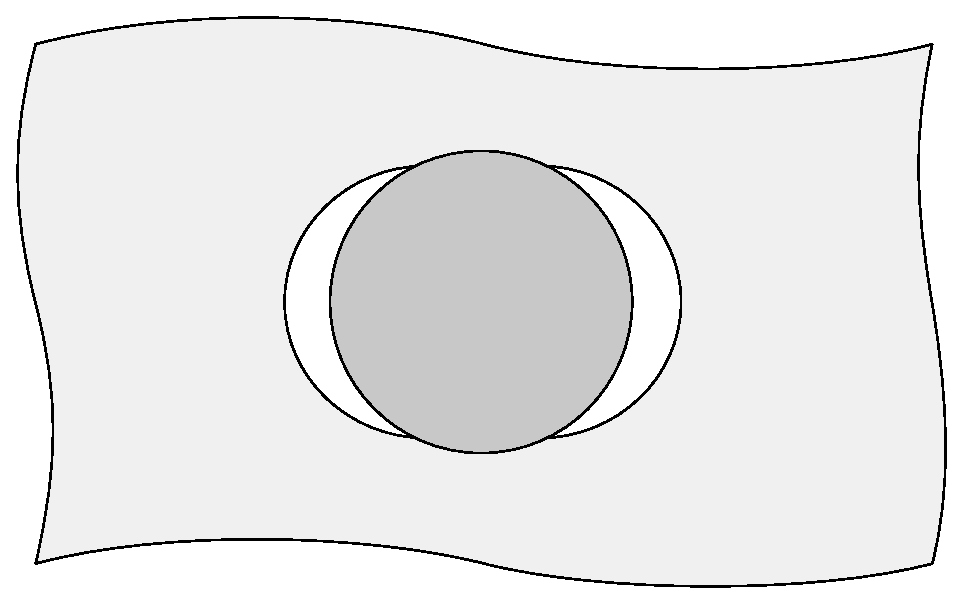
\includegraphics[width=\figwidth,height=\figheight,keepaspectratio]{Obs_Model_Single_Fiber}};
  % Relative node positioning to picture
  % \node[anchor=east] (impactorlabel) at ($(image.west)       + (-0.5cm, 0.5)$) {Impactor};
  % \node[anchor=west] (disklabel)     at ($(image.south east) + ( 0.5cm,0.5)$) {Disk};
  % Figure scope
  \begin{scope}[
    x={(image.south east)},
    y={(image.north west)},
  ]
    
    % Load arrows
    \foreach \y in {0,1,...,\numarrows} {\draw[-latex] (-0.025,\y/\numarrows) -- (-0.1,\y/\numarrows) coordinate (loadarrowleft\y);}
    \foreach \y in {0,1,...,\numarrows} {\draw[-latex] ( 1.025,\y/\numarrows) -- ( 1.1,\y/\numarrows) coordinate (loadarrowright\y);}
    
    % Load label
    \node[anchor=east] (loadlabelleft)  at (loadarrowleft0  |- 0,0.5) {$\glssymbol{symb:scalar:mech:stress:normal:engineering}_x$};
    \node[anchor=west] (loadlabelright) at (loadarrowright0 |- 0,0.5) {$\glssymbol{symb:scalar:mech:stress:normal:engineering}_x$};
    
    % Fibre-Matrix Label
    \node[anchor=south west,inner sep=1pt] (matrixlabel) at (0.05,0.1) {Matrix};
    \node[anchor=north west,inner sep=1pt] (fibrelabel)  at (0.51,0.9) {Fibre};
    \draw[thin] (fibrelabel) -- (0.525,0.725);
    
    % Crack opening
    \draw[thin,latex-latex] (0.66,0.5) -- (0.715,0.5) node[midway,below]{$\glssymbol{symb:scalar:geo:separation}$};
    
    % Fibre diameters
    \draw[dashed] (0.34,0.3) -- (0.34,0.15) coordinate[pos=0.8] (fibrediameterleft);
    \draw[dashed] (0.66,0.3) -- (0.66,0.15) coordinate[pos=0.8] (fibrediameterright);
    \draw[thin,latex-latex] (fibrediameterleft) -- (fibrediameterright) node[midway,below]{$\glssymbol{symb:scalar:geo:diameter}$};
    
    % Help grid and labels
    %\pic{myimagegrid};
  \end{scope}
    
  % Things that are influenced by the aspect ratio
  %\coordinate (fibreorigin) at (0.5,0.5);
  \coordinate (fibreorigin) at ($(image.south east)!0.5!(image.north west)$);
  \draw[thin,dashed] (fibreorigin) -- ++( \failureangle:\fibreradius) coordinate[pos=0.75] (failrt);
  \draw[thin,dashed] (fibreorigin) -- ++(-\failureangle:\fibreradius) coordinate[pos=0.75] (failrb);
  \draw[thin, latex-latex] (fibreorigin) ++(-\failureangle:0.8*\fibreradius) arc (-\failureangle:\failureangle:0.8*\fibreradius) node[midway,left]{$2\glssymbol{symb:scalar:geo:angle:debonding}$};

\end{tikzpicture}
    \tikzexternaldisable
    \caption{Fibre in matrix under transverse load}%\the\figdim \the\figheight 
    \label{fig:Obs:SingleFiber:Model}
  \end{subfigure}%
  \hfill
  \begin{subfigure}{0.39\linewidth}
    % Length
    \setlength{\figwidth}{0.9\linewidth}
    % Figure
    \centering
    \raisebox{\dimexpr.5\ht\largestimage-.5\height}{%
      \tikzexternalenable
      \tikzsetnextfilename{Exp_Fibre_MartyniukK2013}
      %%%%%%%%%%%%%%%%%%%%%%%%%%%%%%%%%%%%%%%
% Header                              %
%%%%%%%%%%%%%%%%%%%%%%%%%%%%%%%%%%%%%%%
% 
% Revisions: 2017-12-12 Martin Raedel <martin.raedel@dlr.de>
%                       Initial draft
%               
% Contact:   Martin Raedel,  martin.raedel@dlr.de
%            DLR Composite Structures and Adaptive Systems
%          
%                                 __/|__
%                                /_/_/_/  
%            www.dlr.de/fa/en      |/ DLR
% 
%%%%%%%%%%%%%%%%%%%%%%%%%%%%%%%%%%%%%%%
% Content                             %
%%%%%%%%%%%%%%%%%%%%%%%%%%%%%%%%%%%%%%%

% \begin{parbox}
\begin{tikzpicture}[
  every node/.style={
    font=\figurefontsize,
  }
]
  % External figure
  \node[anchor=south west,inner sep=0] (image) at (0,0) {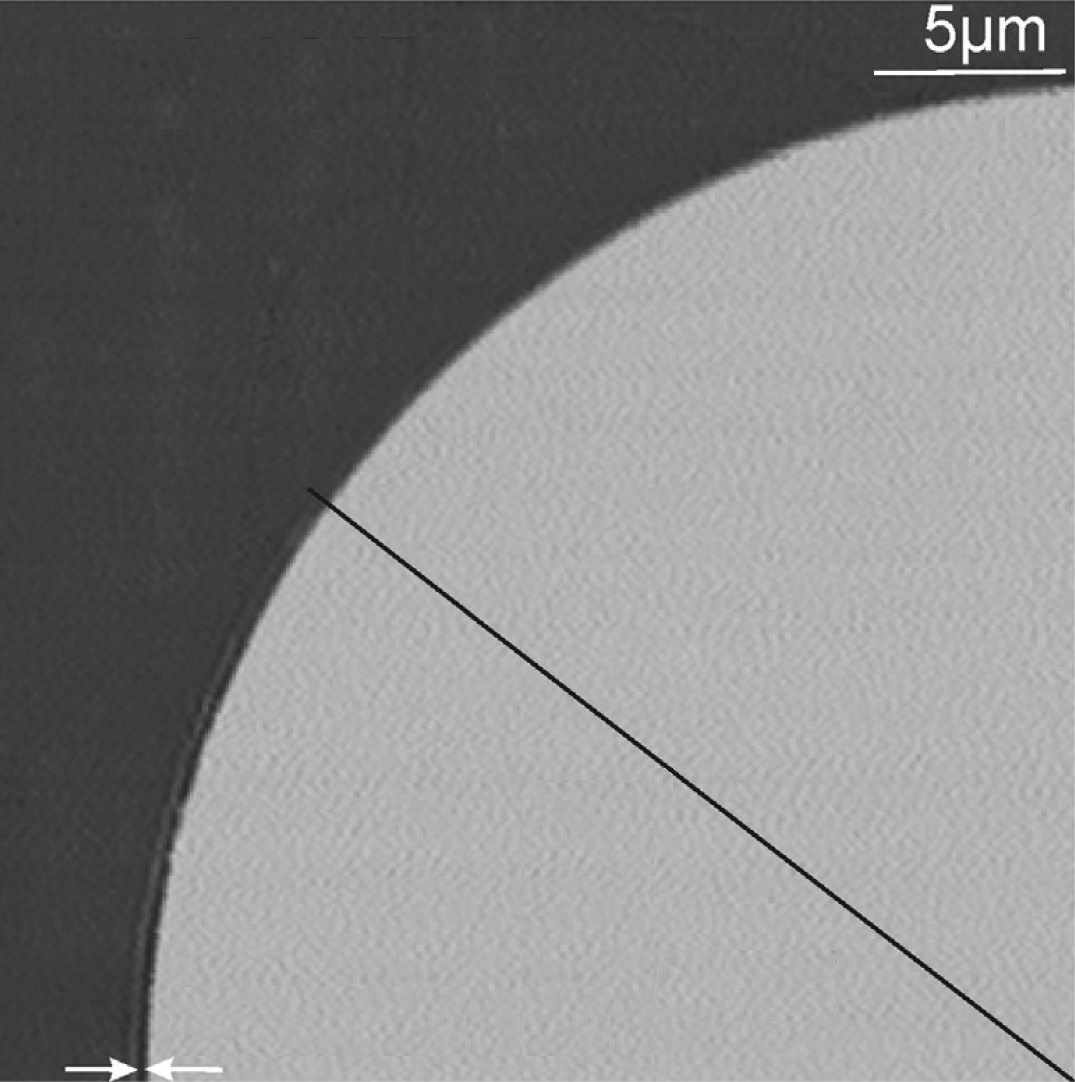
\includegraphics[width=\figwidth,height=\figheight,keepaspectratio]{Exp_Fibre_MartyniukK2013_woLabels2}};
  % Figure scope
  \begin{scope}[
    x={(image.south east)},
    y={(image.north west)},
  ]
    
    \node[anchor=north west,white,inner sep=0pt] (sigmalabel) at (0.025,0.975) {$\glssymbol{symb:scalar:mech:stress:normal:engineering}=\SI{6.2}{\mega\pascal}$};
    
    \node[anchor=south west,black,inner sep=0pt] (deltalabel) at (0.145,0.02) {$\glssymbol{symb:scalar:geo:separation}{=}\SI{0.26}{\micro\meter}$};
    
    %\node[anchor=south east,black,inner sep=0pt] (deltalabel) at (0.85,0.02) {$\glssymbol{symb:scalar:geo:angle:debonding}=\SI{35}{\degree}$};
    
    % This is influenced by the aspect ratio, but since the included graphics is almost square -> hae
    \draw[thin, latex-latex] (1,0) ++(180:0.4) arc (180:142:0.4) node[pos=0.25,right,inner sep=1pt]{$\glssymbol{symb:scalar:geo:angle:debonding}{=}\SI{35}{\degree}$};
    
    % Help grid and labels
    %\pic{myimagegrid};
  \end{scope}
\end{tikzpicture}
      \tikzexternaldisable
    }
    \caption{Experiment}%
    \label{fig:Obs:SingleFiber:Experiment}
  \end{subfigure}%